
Das Visitor Pattern wird eingesetzt um die Operationen aus den Objektstruktur herauszunehmen, um sie erweiterbar zu machen. Die Voraussetzung dafür ist, dass jedes  Element  das Interface \texttt{Element} implementieren um eine Schnittstelle bereitzustellen, die einen Visitor aufnehmen kann. In diesem Fall heißt diese Schnittstelle \texttt{accept(Visitor v}. Das Interface \texttt{Visitor} stellt ihrerseits weitere Schnittstellen zum Besuchen der jeweiligen konkreten Elemente in der Objektstruktur bereit. In diesem Fall wären es zwei Methoden zum besuchen von den konrketen Elementen \texttt{ConcreteElementA} und \texttt{ConcreteElementB}. 
Erhält ein Element einen Visitor, kann er die, für sich bestimmte Methode des Visitors aufrufen. Welche Aktionen diese Methode dann durchführt, kann durch die verschiedenen konkreten Visitors bestimmt werden.

\begin{figure}[htbp]
\centering
%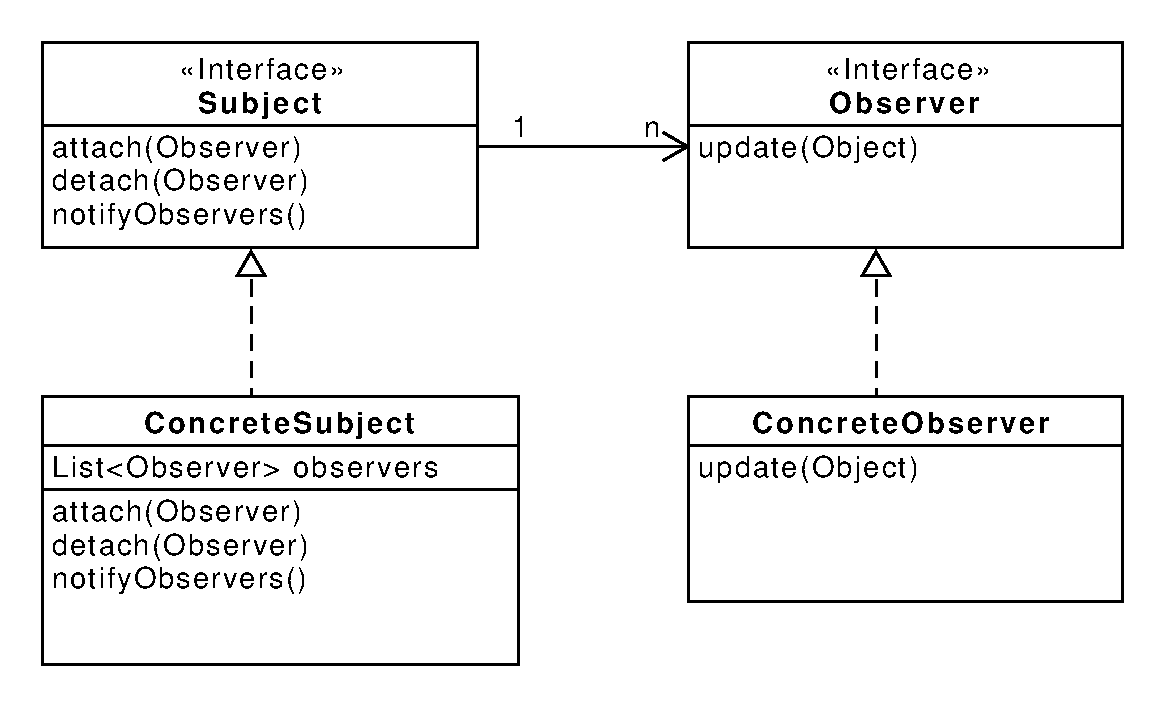
\includegraphics[scale=.5]{./observer/observer}
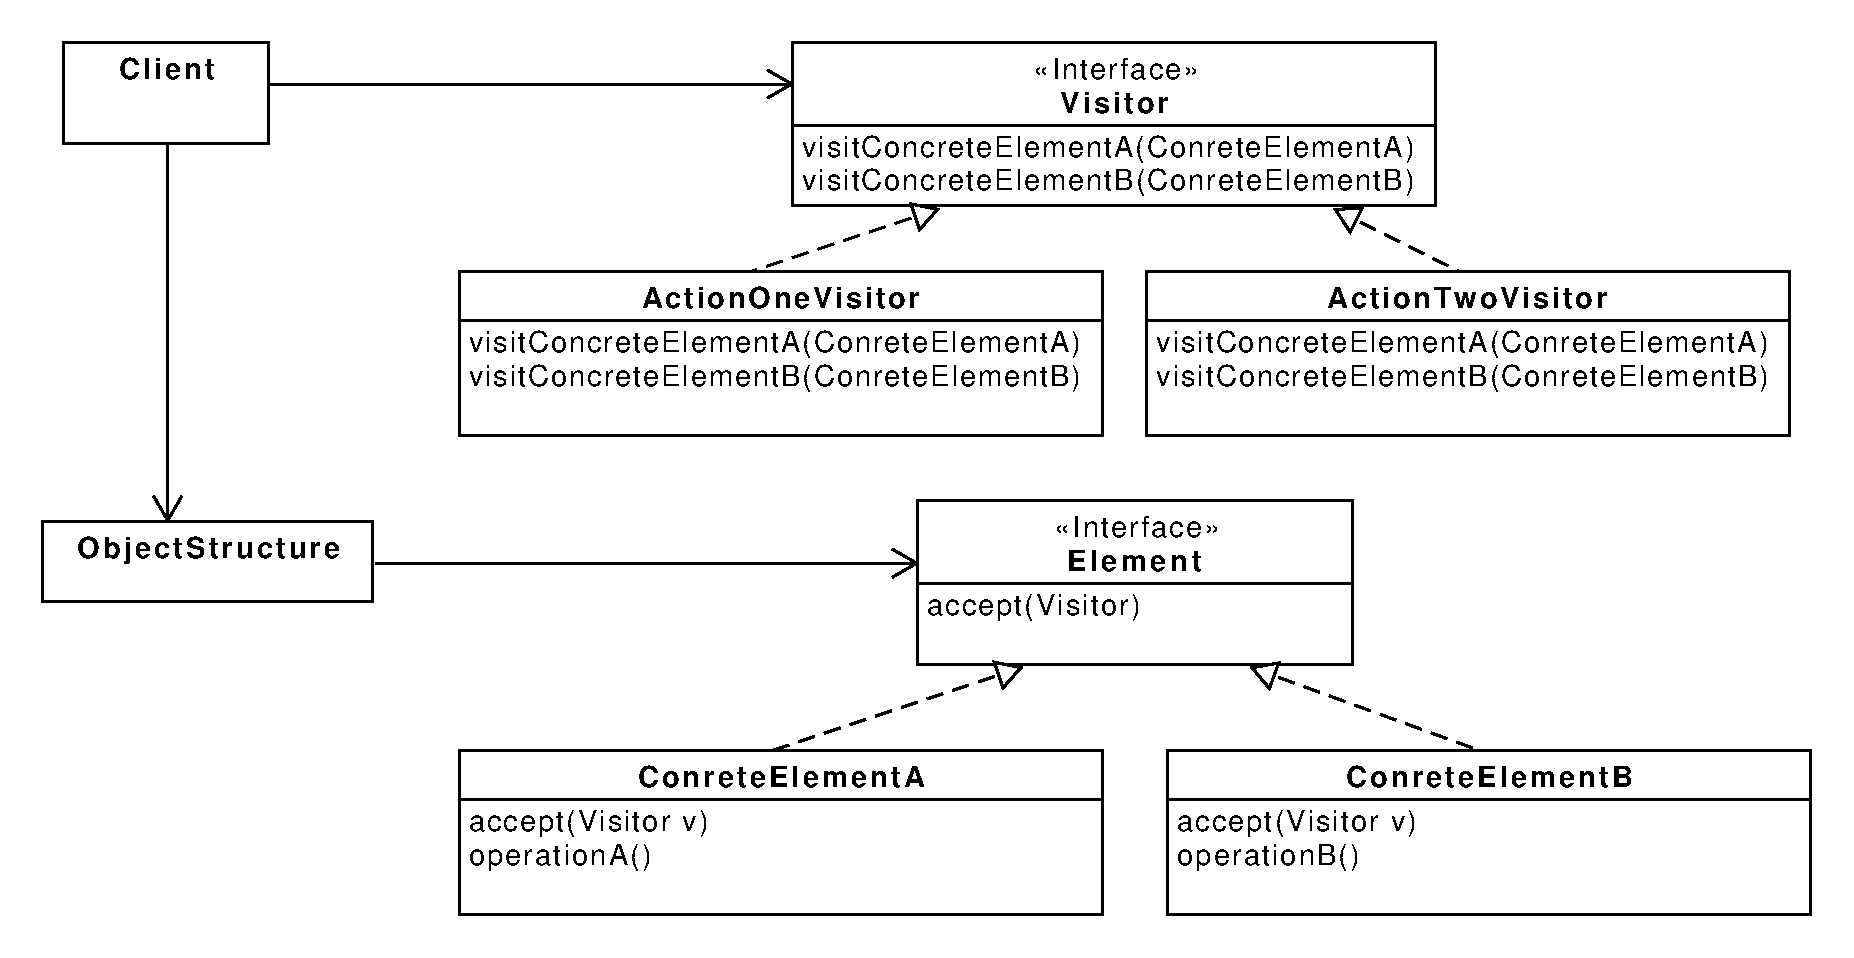
\includegraphics[width=0.9\textwidth]{./paper/visitor/visitor}
\caption{Eine UML-Darstellung von dem Visitor-Pattern.}
\label{observerdiagramm}
\end{figure} 
